\documentclass[14pt,xcolor=pdftex,dvipsnames,table]{beamer}\usepackage[]{graphicx}\usepackage[]{color}
%% maxwidth is the original width if it is less than linewidth
%% otherwise use linewidth (to make sure the graphics do not exceed the margin)
\makeatletter
\def\maxwidth{ %
  \ifdim\Gin@nat@width>\linewidth
    \linewidth
  \else
    \Gin@nat@width
  \fi
}
\makeatother

\definecolor{fgcolor}{rgb}{0.345, 0.345, 0.345}
\newcommand{\hlnum}[1]{\textcolor[rgb]{0.686,0.059,0.569}{#1}}%
\newcommand{\hlstr}[1]{\textcolor[rgb]{0.192,0.494,0.8}{#1}}%
\newcommand{\hlcom}[1]{\textcolor[rgb]{0.678,0.584,0.686}{\textit{#1}}}%
\newcommand{\hlopt}[1]{\textcolor[rgb]{0,0,0}{#1}}%
\newcommand{\hlstd}[1]{\textcolor[rgb]{0.345,0.345,0.345}{#1}}%
\newcommand{\hlkwa}[1]{\textcolor[rgb]{0.161,0.373,0.58}{\textbf{#1}}}%
\newcommand{\hlkwb}[1]{\textcolor[rgb]{0.69,0.353,0.396}{#1}}%
\newcommand{\hlkwc}[1]{\textcolor[rgb]{0.333,0.667,0.333}{#1}}%
\newcommand{\hlkwd}[1]{\textcolor[rgb]{0.737,0.353,0.396}{\textbf{#1}}}%
\let\hlipl\hlkwb

\usepackage{framed}
\makeatletter
\newenvironment{kframe}{%
 \def\at@end@of@kframe{}%
 \ifinner\ifhmode%
  \def\at@end@of@kframe{\end{minipage}}%
  \begin{minipage}{\columnwidth}%
 \fi\fi%
 \def\FrameCommand##1{\hskip\@totalleftmargin \hskip-\fboxsep
 \colorbox{shadecolor}{##1}\hskip-\fboxsep
     % There is no \\@totalrightmargin, so:
     \hskip-\linewidth \hskip-\@totalleftmargin \hskip\columnwidth}%
 \MakeFramed {\advance\hsize-\width
   \@totalleftmargin\z@ \linewidth\hsize
   \@setminipage}}%
 {\par\unskip\endMakeFramed%
 \at@end@of@kframe}
\makeatother

\definecolor{shadecolor}{rgb}{.97, .97, .97}
\definecolor{messagecolor}{rgb}{0, 0, 0}
\definecolor{warningcolor}{rgb}{1, 0, 1}
\definecolor{errorcolor}{rgb}{1, 0, 0}
\newenvironment{knitrout}{}{} % an empty environment to be redefined in TeX

\usepackage{alltt}

% Specify theme
\usetheme{Madrid}
% See deic.uab.es/~iblanes/beamer_gallery/index_by_theme.html for other themes
\usepackage{caption}
\usepackage{tikz}
 \usetikzlibrary{arrows,positioning}
\usepackage[absolute, overlay]{textpos}
\definecolor{MyBrown}{RGB}{180, 151, 90}
\usepackage{multirow}
\usepackage[comma, sort&compress]{natbib}
\usepackage{graphicx}
\graphicspath{{../Pictures/}}
\usepackage{amsmath}
\bibliographystyle{agsm}
% Specify base color
\usecolortheme[named=MyBrown]{structure}
% See http://goo.gl/p0Phn for other colors

% Specify other colors and options as required
\setbeamercolor{alerted text}{fg=Maroon}
\setbeamertemplate{items}[square]
\AtBeginSection[]{
  \begin{frame}
  \vfill
  \centering
  \begin{beamercolorbox}[sep=8pt,center,shadow=true,rounded=true]{title}
    \usebeamerfont{title}\insertsectionhead\par%
  \end{beamercolorbox}
  \vfill
  \end{frame}
}
% Title and author information
\title{Modern Portfolio Theory}
\author{Rob Hayward}
\date{Nov-2016}
\IfFileExists{upquote.sty}{\usepackage{upquote}}{}
\begin{document}

%\begin{frame}
%\titlepage
%\end{frame}

\begin{frame}
\includegraphics[scale=0.4]{FP}
\end{frame}

\begin{frame}
\frametitle{Overview} 
\tableofcontents
\end{frame}

\section{Modern Portfolio Theory}

\begin{frame}{Harry Markowitz}
\begin{center}
\includegraphics[height = 3.0in]{markowitz}
\end{center}
\end{frame}

\begin{frame}{William F. Sharpe}
\begin{center}
\includegraphics[height = 3.0in]{sharpe}
\end{center}
\end{frame}

%\begin{frame}{Merton Miller}
%\begin{center}
%\includegraphics[height = 3.0in]{merton}
%\end{center}
%\end{frame}

\begin{frame}{Modern Portfolio Theory}
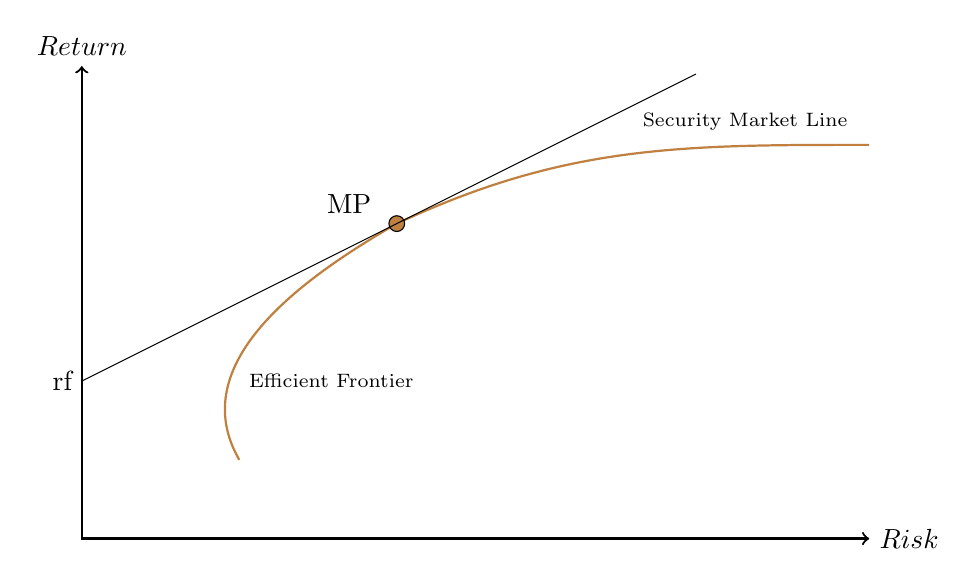
\begin{tikzpicture}[scale = 2] 
%\draw[very thin, color = gray](0, 0) grid (5, 3);
\draw [<->, thick] (0, 3) node (yaxis) [above] {$Return$} 
  |- (5, 0) node (xaxis) [right] {$Risk$};
\pause
\draw[thick, color = brown] (1.0, 0.5) to [out = 120, in = 210] (2.0, 2.0) to [out = 25, in = 180] (5, 2.5);
\node at (1.0, 1.0) [right] {\scriptsize Efficient Frontier};
\pause
\node at (1.9, 2) [above left] {MP};
\draw [fill = brown] (2, 2) circle [radius = 0.05];
\pause
\node at (0, 1) [left] {rf};
\pause
\draw[domain = 0.0:3.9, color = black] plot(\x, {1 + 0.5*\x});
\pause
  \node at (3.5, 2.65) [right] {\scriptsize Security Market Line};
\end{tikzpicture}
\end{frame}

\begin{frame}{Modern Portfolio Theory}
MPT: the \emph{market portfolio} is \emph{mean-variance optimal}
\pause
\vspace{1cm}
\begin{block}{}
Holding the market portfolio is the alternative to forecasting the expected returns and the expected covariances matrix for hundreds of assets
\end{block}
\end{frame}

\begin{frame}{Some questions about MPT}
Some questions about MPT
\begin{itemize}[<+-| alert@+>]
\pause
\item The \emph{investment universe}
\item The market portfolio
\item Expected vs historical record
\item A mean-variance analysis
\item Lack of transaction costs
\item Risk-free asset
\item Stability of relationships
\item Investors are risk-averse
\end{itemize}
\end{frame}
% these may be expanded in slides or just discussion (pictures?)

\begin{frame}{Normal distribution}
\begin{knitrout}
\definecolor{shadecolor}{rgb}{0.969, 0.969, 0.969}\color{fgcolor}
\includegraphics[width=\maxwidth]{figure/norm-1} 

\end{knitrout}
\end{frame}

\begin{frame}{Kurtosis}
\begin{knitrout}
\definecolor{shadecolor}{rgb}{0.969, 0.969, 0.969}\color{fgcolor}
\includegraphics[width=\maxwidth]{figure/kurt-1} 

\end{knitrout}
\end{frame}

\begin{frame}{Skew}
\begin{knitrout}
\definecolor{shadecolor}{rgb}{0.969, 0.969, 0.969}\color{fgcolor}
\includegraphics[width=\maxwidth]{figure/skew-1} 

\end{knitrout}
\end{frame}

\begin{frame}{Black swans}
\centering
\includegraphics[scale = 0.2]{Blackswan}
\end{frame}

\begin{frame}{Unknown unknowns}
\begin{textblock*}{5.2cm}(1cm, 3cm) % (block width) (coords)
\includegraphics[scale = 0.8]{Rumsfeld}
\end{textblock*}
\begin{textblock*}{5.2cm}(6cm, 3cm)
\begin{block}{}
There are things we know; there are things we do not know; there are things that we do not know that we do not know
\end{block}
\end{textblock*}
\end{frame}

%\begin{frame}{Expected values}
\begin{frame}{Capital Asset Pricing Model}
\emph{Capital Asset Pricing Model} (CAPM) is an important part of the MPT framework 
\pause
\begin{itemize}[<+-| alert@+>]
\item There is an public equity risk premium
\item Returns on individual securities is related to this risk premium
\item Beta $(\beta)$ is the measure of this relationship
\begin{itemize}
\item Covariance of asset returns with market returns
\end{itemize}
\item High beta is high risk 
\item Low beta is low risk
\end{itemize}
\end{frame}

\begin{frame}{CAPM}
\begin{tikzpicture}[scale = 2] 
%\draw[very thin, color = gray](0, 0) grid (5, 3);
\draw [<->, thick] (0, 3) node (yaxis) [above] {$Return$} 
  |- (5, 0) node (xaxis) [right] {$Risk$};
\pause
\node at (2.5, 1.75) [below right] {\scriptsize Market Portfolio};
\draw [domain = 0.0:5.0, color = olive] plot(\x, {0.5 + 0.5*\x});
\draw [fill = red] (2.5, 1.75) circle [radius = 0.05];
\pause
\node at (2.5, 1.75) [above left] {$\beta$ = 1};
\end{tikzpicture}
\end{frame}

\begin{frame}{Other risk factors}
A number of additional risk factors have been found
\begin{itemize}[<+-| alert@+>]
\pause
\item \emph{Small cap companies} seem to generate high returns relative to their risk
\item \emph{Value firm} appear to generate high returns relative to their risk
\item \emph{Growth firms} appear to generate low returns relative to their risk
\item There are other \emph{risk factors} or anomalies that we will return to later
\end{itemize}
\end{frame}

\begin{frame}{CAPM}
\begin{tikzpicture}[scale = 2] 
%\draw[very thin, color = gray](0, 0) grid (5, 3);
\draw [<->, thick] (0, 3) node (yaxis) [above] {$Return$} 
  |- (5, 0) node (xaxis) [right] {$Risk$};
\pause
\draw[domain = 0.0:5.0, color = olive] plot(\x, {0.5 + 0.5*\x});
\draw [fill = brown] (2.5, 1.75) circle [radius = 0.05];
%\node at (2.5, 1.75) [above left] {$\beta$ = 1};
\node at (2.5, 1.75) [below right] {\scriptsize Market Portfolio};
\pause
\draw [fill = brown] (3.5, 2.5) circle [radius = 0.05];
\node at (3.5, 2.5) [left] {\scriptsize Small Capitalisation};
\pause
\draw [fill = brown] (1.5, 1.5) circle [radius = 0.05];
\node at (1.5, 1.5) [left] {\scriptsize Value};
\pause
\draw [fill = brown] (3.5, 2.0) circle [radius = 0.05];
\node at (3.5, 2.0) [right] {\scriptsize Growth};
\end{tikzpicture}
\end{frame}

\section{Passive vs Active investment}
\begin{frame}{Economist and the one hundred dollar bill}
\begin{center}
\includegraphics[scale = 0.06]{oneHundredDollar}
\end{center}
\end{frame}

\begin{frame}{Market efficiency}
The Efficient Market Hypothesis 
\begin{itemize}[<+-| alert@+>]
\pause
\item Suggests that inefficiencies will be swiftly eliminated
\item There are no \emph{systematic} deviations that allow \emph{supernormal profits} or returns that are more than just compensation for risk
\item Are these effects (value, growth etc) inefficiencies or risk factors? 
\end{itemize}
\end{frame}

\begin{frame}{Value Investment}
\frametitle{Value investment}
\begin{center}
\includegraphics[height = 3.0in]{BGsmall}
\end{center}
\end{frame}

\begin{frame}{Active investment}
Active funds try to take advantage of these apparent inefficiencies
\begin{itemize}[<+-| alert@+>]
\pause
\item \emph{Value Investment}
\begin{itemize}
\item Benjamin Graham
\item Warren Buffett
\item Berkshire Hathaway
\end{itemize}
\item Security selection
\begin{itemize}
\item Stock, bond, commodity or country
\end{itemize}
\item Hedge funds
\begin{itemize}
\item Range of strategies to capture \emph{alpha} or to find \emph{absolute returns} that are not correlated highly with the market 
\end{itemize}
\end{itemize}
\end{frame}

\begin{frame}{Active management success}
\begin{itemize}[<+-| alert@+>]
\pause
\item Many studies find that active managers are not successful on average
\begin{itemize}
\item Malkiel (1995), Gruber (1996), Wermers (2000, 2003), and Jones
and Wermers (2011)
\end{itemize}
\item However, individual managers may be successful
\item Hedge funds have come under increased scrutiny and questions are raised about high fees
\end{itemize}
\end{frame}
 
\begin{frame}{Rise of Passive Investment}
\textbf{Morningstar}
\begin{itemize}[<+-| alert@+>]
\pause
\item Index-tracking funds increased share by \$2.0trn since 2013, reaching \$5.0tn
\item Dominated by Vanguard and BlackRock in US equity market
\item Only 16.9\% of US large-growth managers were able to beat their passive counterparts over the 10 year period
\item Cost is a major contributor to investment performance
\item Hedge funds notoriously charge 2\% and 20\%
\end{itemize}
\end{frame}

\section{Portfolio construction: decision-making}
%\begin{frame}{Fund structure and performance}
%There are two main structures for funds
%\begin{itemize}[<+-| alert@+>]
%\pause
%\item Endowment model
%\begin{itemize}
%\item Strategic asset allocation
%\item Asset holdings are changed gradually
%\item Performance measured against asset benchmark
%\end{itemize}
%\item Opportunity cost model
%\begin{itemize}
%\item Benchmark is a passive investment in stocks and bonds
%\item Leeway for fund managers to buy alternative assets (but tracking-error limits)
%\item Performance (net of fees) is judged against benchmark
%\end{itemize}
%\end{itemize}
%\end{frame}

\begin{frame}{Portfolio construction}
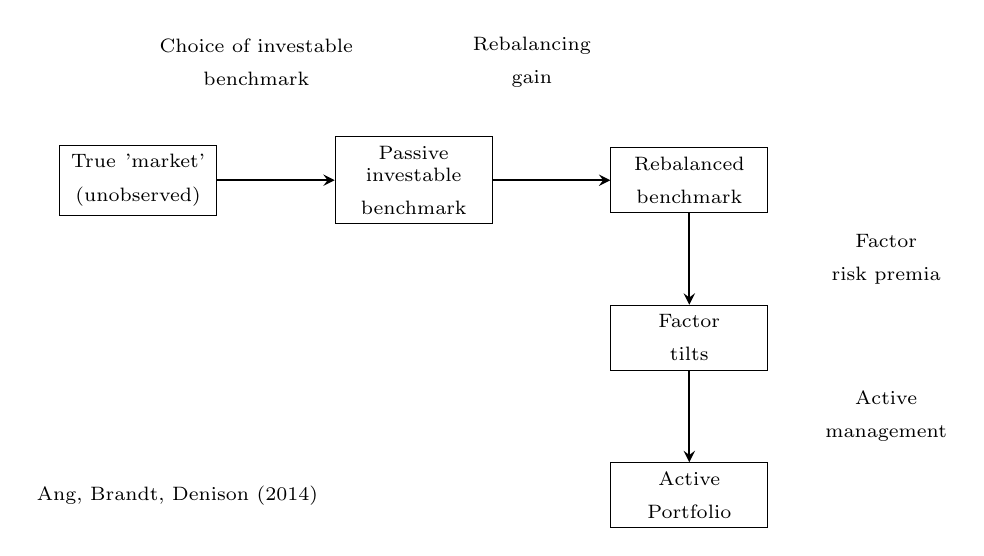
\begin{tikzpicture} 
%\draw[very thin, color = gray](0, 0) grid (12, 6);
\tikzstyle{block} = [draw, rectangle, text width = 5em, 
  text centered, minimum height = 6mm, node distance = 5em];
\tikzstyle{line} = [draw, -stealth, thick]
\node [block] at (1.5, 4) (one) {\scriptsize True 'market' \\ (unobserved)};
\node [block] at (5, 4) (two) {\scriptsize Passive investable \\ benchmark};
\node [block] at (8.5, 4) (three) {\scriptsize Rebalanced \\ benchmark};
\node [block] at (8.5, 2) (four) {\scriptsize Factor \\ tilts};
\node [block] at (8.5, 0) (five) {\scriptsize Active \\ Portfolio};
\path [line] (one) -- (two);
\path [line] (two) -- (three);
\path [line] (three) -- (four);
\path [line] (four) -- (five);
\node at (3, 5.5) [align = center]{\scriptsize Choice of investable \\ \scriptsize benchmark};
\node at (6.5, 5.5) [align = center]{\scriptsize Rebalancing \\ \scriptsize gain};
\node at (11, 3) [align = center] {\scriptsize Factor \\ \scriptsize risk premia};
\node at (11, 1) [align = center] {\scriptsize Active \\ \scriptsize management};
\node at (2, 0) [align = center] {\scriptsize Ang, Brandt, Denison (2014)};
\end{tikzpicture}
\end{frame}

\begin{frame}{Active components of fund}
There are a number of places where the fund must be active
\begin{itemize}[<+-| alert@+>]
\pause
\item Deciding on the appropriate market
\item Finding an investable fund
\item Frequency of asset re-balancing
\item Factor tilts
\item Active security selection
\end{itemize}
\end{frame}

\begin{frame}{Norwegian Petroleum Fund}
\begin{center}
\includegraphics[height = 3.0in]{Flag_Norway}
\end{center}
\end{frame}

\begin{frame}{Norwegian Petroleum Fund}
Started in 1996 with NOK 40 bn now has 7.2tn (\$875bn) 
\begin{itemize}[<+-| alert@+>]
\pause
\item 1998 - 40\% of assets were equities
\item 2001 - Budetary rule (maximum of 4\% to be used)
\item 2009 - 60\% of assets were equities
\item 2010 - 5\% real estate
\item Today 60\% equity, 35\% fixed income, 5\% real estate
\item Ethical council 
\item Mork Committee
\end{itemize}
\end{frame}

\begin{frame}{Knut Anton Mork}
\begin{center}
\includegraphics[height = 3.0in]{mork}
\end{center}
\end{frame}

\begin{frame}{Mork}
Committee was split
\begin{itemize}[<+-| alert@+>]
\pause
\item Majority wants to increase equity share to 70\%
\begin{itemize}
\item Risky oil and gas reserves have fallen as a share of assets
\item Fiscal rule could be more adaptable
\end{itemize}
\item Mork wants to reduce the size of the equity share to 50\%
\begin{itemize}
\item Concerned about the need for steady fiscal transfers
\end{itemize}
\end{itemize}
\end{frame}



%\section{Portfolio Practice}
%\begin{frame}{Portfolio Practice}
%Research and sales focus on (US) stocks, but $\dots$
%\begin{itemize}[<+-| alert@+>]
%\pause
%\item Diversification for bonds
%\begin{itemize}
%\item Diversify across levels of credit
%\item Diversify across maturities
%\item Diversify across countries
%\end{itemize}
%\item Diversification for commodities
%\item Diversification for currency
%\end{itemize}
%\end{frame}
%
%\begin{frame}{Bonds}
%Two big issues for bond markets
%\begin{itemize}[<+-| alert@+>]
%\pause
%\item Hordahl et al. (2016): 2005-15 100bp rise in US yield curve associated with a 70bp to 80bp rise in  
% \item Reduced liquidity due to regulation of investment banks (rebalancing more expensive)
% \item Increased use of ETF in the second (article on feedly)
% \end{itemize}
% \end{frame}


\section{Smart Beta}
\begin{frame}{Criticisms of index investment}
There are a number of persistent criticisms of using traditional indices as the basis for investment
\begin{itemize}[<+-| alert@+>]
\pause
\item An index may not be available (non-investable)
\item Index investment impedes the process of \emph{price discovery}
\item Capitalisation-weighted indices are \textbf{NOT} equivalent to the \emph{market portfolio}
\begin{itemize}
\item Weights must be increased as shares gain in price
\item Causes investors to buy \emph{winning stocks} and sell \emph{losing stocks}
\item Buy \emph{growth} and sell \emph{value}
\item Overweight over-valued and under-weight undervalued
\end{itemize}
 
\end{itemize}
\end{frame}

\begin{frame}{Smart Beta}
There are two main types of Smart Beta:
\begin{itemize}[<+-| alert@+>]
\pause
\item Take \emph{value-weighted} indices and weight them by some other measure
\item Use risk \emph{factors} or anomalies 
\end{itemize}
\end{frame}

\begin{frame}{Fundamental indexation}
%\begin{textblock*}{3cm}(1cm, 1.5cm)
%\includegraphics[scale = 0.3]{RA}
%\end{textblock*}
Research Affiliates is generally credited with introducing the first \emph{Smart Beta} fund 
\begin{itemize}[<+-| alert@+>]
\pause
\item Arnott, R., J. Hsu and P. Moore, \emph{Fundamental Indexation}, Financial Analysts Journal, 2005
\item Fundamentally-weight index fund was launched in 2005. 
\item \textbf{RAFI}
\end{itemize}
\end{frame}

\begin{frame}{Fundamentally weighted indices}
\begin{columns}{}
\begin{column}{0.48\linewidth}
\includegraphics[scale = 0.38]{Main-Street}
\end{column}
\begin{column}{0.47\linewidth}
\includegraphics[scale = 0.18]{Wall-Street}
\end{column}
\end{columns}
\end{frame}

\begin{frame}{Fundamentally weighted indices}
Arnott, Hsu and More tested a range of alternative (fundamental) weightings
\begin{itemize}[<+-| alert@+>]
\pause
\item Book value
\item Trailing 5-year average cash flow
\item Trailing 5-year average revenue
\item Trailing 5-year average gross sales
\item Trailing 5-year average gross dividends
\item Total employment
\item Composite of book, cash-flow, sales and dividends (most widely available for most countries)
\end{itemize}
\end{frame}

\begin{frame}{Details}
\begin{itemize}[<+-| alert@+>]
\item Compustat data from 1962 to 2004
\item Portfolio re-balanced once a year (at end of year)
\item Comparison of expansion and recession
\item Comparison of rising and falling interest rate environments
\end{itemize}
\end{frame}

\begin{frame}{Fundamentally weighted indices: results}
\begin{table}
\begin{center}
\rowcolors{1}{MyBrown!20}{MyBrown!5}
\begin{tabular}{l r r r}
\textbf{Portfolio/index} & \textbf{1980s} & \textbf{1990s} & \textbf{2000-04}\\
\hline
S\&P 500 & 17.7\% & 18.6\% & -2.1\% \\
Book & 18.3\%     & 17.1\% & 5.8\%\\
Income & 19.0\%   & 17.7\% & 7.6\% \\
Sales & 19.5\%    & 16.8\% & 8.7\% \\
Dividends & 19.2\% & 15.4\% & 8.0\% \\
Employment & 17.7\% & 15.7\% & 7.8\%\\
Composite & 19.0\% & 16.6\% & 7.7\% 
\end{tabular}
\end{center}
\end{table}
Annualised returns by decade.  Arnott, Hsu and More (2005)
\end{frame}

\begin{frame}{Fundamentally-weighted index}
\begin{itemize}[<+-| alert@+>]
\item Is this \emph{data mining}?
\begin{itemize}
\item Based on fundamental measures of company size
\item Results hold across decades 
\item Results hold across expansions and contractions
\item Results hold in rising and falling rate environment
\end{itemize}
\item Choosing individual value and growth companies is difficult
\item Here \emph{market inefficiencies} are found on average
\end{itemize}
\end{frame}

\begin{frame}{Comparison with capitalisation-weighted investment}
You have the advantages of the \emph{capitalisation-weighted} investment without the costs
\begin{itemize}[<+-| alert@+>]
\pause
\item It is a passive strategy with natural re-weighting
\item Large stocks have the largest weight
\begin{itemize}
\item This means high liquidity and low trading costs
\end{itemize}
\item Correlation with the returns and volatility of the capitalisation-weighted index is high
\end{itemize}
\end{frame}

\begin{frame}{Comparison to Capitalisation-weighed index (2000-04)}
%\begin{center}
\rowcolors{1}{MyBrown!20}{MyBrown!5}
\begin{table}
\begin{center}
\begin{tabular}{l r r r}
\textbf{Portfolio/index} & \textbf{Value-added} & \textbf{Std Dev} &  \textbf{Sharpe}\\
\hline
S\&P 500 & -0.43pp & 18.0\%& 0.27 \\
Book &      7.57pp&  18.2\%& 0.17\\
Income &    9.33pp&  17.5\%& 0.28 \\
Sales &     10.4pp&  18.2\%& 0.31 \\
Dividends & 9.71pp&  15.3\%& 0.35 \\
Employment & 9.55pp& 18.6\%& 0.28\\
Composite &  9.32pp& 17.2\%& 0.28 
\end{tabular}
\end{center}
\end{table}
Value-added and risk adjusted returns.  Arnott, Hsu and More (2005)
\end{frame}

\section{Factor investment}
\begin{frame}{Factor investment}
Fundamentally-weighted indices would tend to pick up the value and growth anomalies: Ang, Goetzmann and Schaefer (2009)
\begin{itemize}[<+-| alert@+>]
\pause
\item They may even pick up some of the small-cap anomaly
\item Investors have sought to systematically capture others
\begin{itemize}
\item Momentum
\item Low volatility 
\item Quality
\end{itemize}
\end{itemize}
\end{frame}

\begin{frame}{CAPM}
\begin{tikzpicture}[scale = 2] 
%\draw[very thin, color = gray](0, 0) grid (5, 3);
\draw [<->, thick] (0, 3) node (yaxis) [above] {$Return$} 
  |- (5, 0) node (xaxis) [right] {$Risk$};
\pause
\draw[domain = 0.0:5.0, color = olive] plot(\x, {0.5 + 0.5*\x});
\draw [fill = brown] (2.5, 1.75) circle [radius = 0.05];
%\node at (2.5, 1.75) [above left] {$\beta$ = 1};
\node at (2.5, 1.75) [below right] {\scriptsize Market Portfolio};
\pause
\draw [fill = brown] (3.5, 2.5) circle [radius = 0.05];
\node at (3.5, 2.5) [left] {\scriptsize Small Capitalisation};
\pause
\draw [fill = brown] (1.5, 1.5) circle [radius = 0.05];
\node at (1.5, 1.5) [left] {\scriptsize Value};
\pause
\draw [fill = brown] (3.5, 2.0) circle [radius = 0.05];
\node at (3.5, 2.0) [right] {\scriptsize Growth};
\end{tikzpicture}
\end{frame}

\begin{frame}{Factor investment}
\begin{table}
\begin{center}
\rowcolors{1}{MyBrown!20}{MyBrown!5}
\begin{tabular}{l r r }
\textbf{Factor} & \textbf{What is it?} & \textbf{Metric} \\
\hline
Value & Cheap & Book-to-price\\
Size & Small cap & Capitalisation\\
Momentum & Past performance & Recent gains\\
Low vol & Low risk & Standard deviation\\
Dividend & High dividend & Dividend yield\\
Quality & Robust & Debt or management\\
\end{tabular}
\end{center}
\end{table}
Most common factors, what they are and how they can be measured
\end{frame}

\begin{frame}{Factor risks}
\begin{itemize}[<+-| alert@+>]
\pause
  \item \textbf{Value:} behavioural bias of pro-cyclical investment: De Bondt and Thaler (1985) and Fama French (1993)
\item \textbf{Growth:} behavioural bias of pro-cyclical investment: De Bondt and Thaler (1985) and Fama French (1993)
\item \textbf{Small cap:} increased risk of small firms, liquidity or access to funding: Fama French (1993)
\item \textbf{Momentum:} behavioural and institutional serial correlation: Jagadesh and Titman (1993)
\item \textbf{Volatility:} Black, Jensen and Scholes (1972)
\item \textbf{High dividend:}
\item \textbf{Quality:} 
\end{itemize}
\end{frame}

\begin{frame}{Results of factor investment}
Investec analysis of following factors for S\&P 500 and MSCI EAFE (Dec 1991 to Dec 2015)
\begin{itemize}[<+-| alert@+>]
\pause
\item \textbf{Value:} 20\% of stocks with the lowest price-to-book ratio
\item \textbf{Small tilt:} 20\% with smallest capitalisation
\item \textbf{Momentum:} 20\% with the highest 12-month price return
\item \textbf{Low volatility:} 20\% with the lowest 12-month realised volatility
\item \textbf{Quality:} top 20\% of stocks with highest rating for return on equity, debt-to-equity and earnings variability
\end{itemize}
\end{frame}

\begin{frame}{Results 1}
Dec 1991 to Dec 2015
%\begin{center}
\rowcolors{1}{MyBrown!20}{MyBrown!5}
\begin{table}
\begin{center}
\begin{tabular}{l r r }
\textbf{Portfolio/index} & \textbf{Return} & \textbf{Risk-adjusted return} \\
\hline
S\&P 500        & 9.0\% &  0.6\\
Quality         & 11.1\% & 0.8\\
Value           & 10.6\% & 0.5\\
Small tilt      & 13.9\% & 0.6\\
Momentum        & 12.0\% & 0.8\\
Low volatility &  10.5\% & 0.9\\
\end{tabular}
\end{center}
\end{table}
US stocks; risk-adjusted return is return per unit of volatility. Bender, Briand, Melas, Subramanian (2013)
\end{frame}

\begin{frame}{Results 2}
Dec 1991 to Dec 2015
%\begin{center}
\rowcolors{1}{MyBrown!20}{MyBrown!5}
\begin{table}
\begin{center}
\begin{tabular}{l r r }
\textbf{Portfolio/index} & \textbf{Return} & \textbf{Risk-adjusted return} \\
\hline
MSCI EAFA        & 4.7\% &  0.3\\
Quality         & 9.7\% & 0.7\\
Value           & 9.5\% & 0.5\\
Small tilt      & 7.9\% & 0.4\\
Momentum        & 9.0\% & 0.6\\
Low volatility &  10.0\% & 0.8\\
\end{tabular}
\end{center}
\end{table}
International stocks; risk-adjusted return is return per unit of volatility. Bender, Briand, Melas, Subramanian (2013).
\end{frame}
% Barra Risk models also inclue liqudiity and growth but these do not 
% produce excess retruns over the long-run. 
% Do we use the next slide or put some of this information in the sliede abovve



\begin{frame}{Fixed income}
Enthusiasm for factor investment has spread from equities to other asset classes, including bonds
\begin{itemize}[<+-| alert@+>]
\pause
\item Fama-French (1993) includes maturity and default risk factors for bonds
\item However, of 573 funds in Morning Star Strategic Beta universe, only 19 are fixed income
\item Bonds already have a layer of active investment (maturing bonds must be replaced)
\item There is less reliable data for identifying factors
\item Over-the-counter market makes pricing less reliable or transparent
\end{itemize}
\end{frame}

\begin{frame}{Fixed income and capitalisation}
Capitalisation is even more a problem with fixed income
\begin{itemize}[<+-| alert@+>]
\pause
\item GDP-weighted indices compared to market-capitalisation
\item Research Affiliates also have
\begin{itemize}
\item population
\item land area
\item energy consumption
\end{itemize}
\item Lower liquidity may reduce the frequency of rebalancing 
\end{itemize}
\end{frame}

\begin{frame}{Fundamental factors}
These are for government and corporate sectors
\begin{itemize}[<+-| alert@+>]
\pause
\item Government 
\begin{itemize}
\item deficit-to-GDP
\item debt-to-GDP
\item demographics and political stability
\end{itemize}
\item Corporate 
\begin{itemize}
\item free cash flow 
\item leverage
\end{itemize}
\item Equity-like factors
\begin{itemize}
\item Value, size, momentum, volatility, quality
\end{itemize}
\item Other
\begin{itemize}
\item term, liquidity, credit 
\end{itemize}  
\end{itemize}
\end{frame}

\begin{frame}{Factors in Norwegian oil fund}
Ang, Goetzmann and Schaefer (2009) find the following factors explain the active activity of fund
\begin{itemize}[<+-| alert@+>]
\pause
\item \textbf{Term:} yield curve 
\item \textbf{Credit:} credit risk
\item \textbf{FX carry:} carry-trade
\item \textbf{Liquidity:} purchase is illiquid assets
\item \textbf{Value-growth:} long-value/short-growth
\item \textbf{Size:} long-small cap/short-large cap
\item \textbf{Momentum:} Buy recent winners sell recent losers
\item \textbf{Vol:} Spread between implied and realised volatility
\end{itemize}
\end{frame}
\section{Other methods portfolio methods}
\begin{frame}{Assets as bundles of risk}
\begin{textblock*}{5cm}(1cm, 2cm)
Colourful metaphor
\end{textblock*}
\begin{textblock*}{5.2cm}(1cm, 3cm) % (block width) (coords)
\includegraphics[scale = 0.1]{vit}
\end{textblock*}
\begin{textblock*}{5.2cm}(6.5cm, 3cm)
\includegraphics[scale = 0.6]{atom}
\end{textblock*}
\end{frame}

\begin{frame}{Assets as bundles of risk}
For a standard pension fund (adapted from Podkaminer (2013) CFA Institute)
\begin{table}
\begin{center}
\rowcolors{1}{MyBrown!20}{MyBrown!5}
\begin{tabular}{l r r r}
\textbf{Asset} & \textbf{\%} & \textbf{Risk} & \textbf{\%}\\
\hline
US equity     & 25\% & Equity & 57\% \\
Non-US equity & 10\% & & \\
Emerging equity & 2\% & & \\
Private equity  & 20\% &  &  \\
\hline
US fixed income & 20\% & Interest rate&  10\%\\
Global fixed income & 5\% & Credit & 18\%\\
Cash            & 3\% & &  \\

Real estate     & 10\% & Real estate & 10\%\\
Other           & 5\% & Other & 5\% \\
\end{tabular}
\end{center}
\end{table}

\end{frame}


\begin{frame}{Risk parity}
Weight assets so that their risk to the portfolio is equal.  
\begin{itemize}[<+-| alert@+>]
\pause
%\item All-Weather Asset-allocation approach introduced by Bridgewater
\item The large variance of equities usually dominates a 60/40 portfolio
\item A 25/75 equity-bond mix will equalise effects of each asset but will reduce the expected return
\item Leveraging bonds to have a risk that is comparable to equities will reduce the overall risk of portfolio \textbf{and} increase the expected return
\item This takes advantage of \emph{leverage aversion}
\item There is risk that is not quantified
\end{itemize}
\end{frame}

\begin{frame}{Risk parity examples}
\begin{table}
\begin{center}
\rowcolors{1}{MyBrown!20}{MyBrown!5}
\begin{tabular}{l  p{2.5cm} r}
\textbf{Performance} & \textbf{60/40 stock-bonds} & \textbf{Risk parity}\\
\hline
Total Return & 8.5\% & 10.4\% \\
Excess Return & 4.1\% & 5.9\%\\
Standard Deviation & 8.9\% & 8.3\% \\
Sharpe Ratio & 0.45 & 0.72
\end{tabular}
\end{center}
\end{table}
Risk-parity vs traditional average 1946 to 2015: Dalio, Prince, Jensen (2015)
\end{frame}

\begin{frame}{Other methods}
\begin{itemize}[<+-| alert@+>]
\pause
\item Matching liabilities 
\begin{itemize}
\item Treat liabilities as a short position to be hedged
\item Maturity matching
\item Are liabilities bond-like or equity-like?
\end{itemize}
\item Statistical methods
\begin{itemize}
\item Principal components (PCA)
\item Seeks to identify orthogonal factors that contribute most to the variation of the portfolio
\end{itemize}
\end{itemize}
\end{frame}

%\begin{frame}{Statistical factors}
%It is also possible to use statistical methods to draw out factors
%\begin{itemize}[<+-| alert@+>]
%\pause
%\item Principal components analysis (PCA)
%\end{itemize}
%\end{frame}
%
\section{Criticism}
\begin{frame}{Criticisms of Smart Beta and Factor Investment}
There are a number of criticism of Smart Beta (ironically, these have recently 
come from \textbf{Research Affiliates}). 
\begin{itemize}[<+-| alert@+>]
\pause
\item Data mining
\item Exploitation of the inefficiency should remove that inefficiency
\item Factors depend on underlying economic conditions
\item Factors can become crowded or expensive 
\end{itemize}
\end{frame}

\begin{frame}{Torture the data until it speaks}
\begin{center}
\includegraphics[height = 3.0in]{torture}
\end{center}
\end{frame}

\begin{frame}{But...}
Behavioural studies find that it is natural to seek patterns
\pause
\vspace{1cm}
\begin{block}{}
Even when they do not exist!
\end{block}
\end{frame}

\begin{frame}{Patterns emerge}
\begin{center}
\includegraphics[scale = 0.35]{jesus-clouds}
\end{center}
\end{frame}


\begin{frame}{Increased efficiency}
R. Arnott studied performance of factors before and after publication
\begin{itemize}[<+-| alert@+>]
\pause
\item 8 published factors since 1967
\item Return of 5.8\% before publication
\item Return of 2.6\% after publication
\end{itemize}
\end{frame}

\begin{frame}{Economist and the one hundred dollar bill}
\begin{center}
\includegraphics[scale = 0.06]{oneHundredDollar}
\end{center}
\end{frame}

\begin{frame}{Factors are expensive}
Recent work by Research Affiliates finds that factors have become \emph{expensive}
\begin{itemize}[<+-| alert@+>]
\pause
\item Assess whether factors are expensive of cheap by measuring the price-to-book ratio
\item Compare the value (price-to-book) vs 5 year returns
\item Find the current valuation
\item Changes in recent years  may be driven by valuation
\end{itemize}
\end{frame}

\begin{frame}{Factor value}
\begin{table}
\begin{center}
\rowcolors{1}{MyBrown!20}{MyBrown!5}
\begin{tabular}{l  p{2.3cm} r}
\textbf{Testing} & \textbf{Coefficient} & \textbf{Current value}\\
\hline
Value vs growth & -1.9\%* & Cheap\\
Capitalisation & -0.72\%* & Mid\\
Momentum & -0.34\%* & Cheap\\
Liquidity & -0.45\%* & Expensive\\ 
Beta & -0.00 & Cheap\\
Profitable & -0.35\%* & Expensive\\
\end{tabular}
\end{center}
\end{table}
Factor valuation vs following 5-year returns.  1967-2015.  R. Arnot, N. Beck, V. Kalesnik and J. West, Feb 2016.  
* Statistically significant
\end{frame}

\begin{frame}{For example: Low volatility}
These have been one of the biggest winners of 2016
\begin{itemize}[<+-| alert@+>]
\pause
\item Introduced in 2011
\item BlackRock USMW 
\item Inflow of \$16.0bn in first 9 months of 2016
\item 28 funds hold \$44bn in assets (XTF)
\item Seek to identify boring stocks.  
\item Low or minimal volatility
\item Tend to be high dividend stocks
\item \emph{Crowded?} - concentrated in utilities
\end{itemize}
\end{frame}


\begin{frame}{Fickle Factors}
How resilient are these factors? 
\begin{itemize}[<+-| alert@+>]
\pause
\item What is the source of the factor \emph{excess return}?
\begin{itemize}
\item Increased risk
\item Inefficiency
\begin{itemize}
\item behavioural
\item institutional
\end{itemize}
\end{itemize}
\item Will the returns continue? 
\end{itemize}
\end{frame}

\begin{frame}{Factor source 1}
\begin{table}
\begin{center}
\rowcolors{1}{MyBrown!20}{MyBrown!5}
\begin{tabular}{l l l}
\textbf{Factor} & \textbf{Risk} & \textbf{Behavr-Instit}\\
\hline
\textbf{Value} & Systematic risk & Expectation error\\
      &                 & Loss aversion\\
      &                 & Investment flows\\
\textbf{Size}  & Systematic risk & Expectation error\\
      & Liquidity risk   & \\
\textbf{Momentum} & Crash risk & Over-reaction\\
        &             & Investment flows\\
        &             & Asynchronous trade\\
\end{tabular}
\end{center}
\end{table}
%Adapted from MSCI \emph{Foundations of Factor Investment}

\end{frame}

\begin{frame}{Factor source 2}
\begin{table}
\begin{center}
\rowcolors{1}{MyBrown!20}{MyBrown!5}
\begin{tabular}{l p{3cm} l}
\textbf{Factor} & \textbf{Risk} & \textbf{Behavr-Instit}\\
\hline
\textbf{Low vol} & NA          & Lottery effect\\
        &             & Overconfidence\\
        &             & Leverage aversion\\
\textbf{Quality} & NA          & Expectations errors\\
        &             & Manipulated earnings\\
\end{tabular}
\end{center}
\end{table}
Adapted from MSCI \emph{Foundations of Factor Investment}

\end{frame}



\section{The future}
\begin{frame}{Low rate world}
State street conducted a survey of the portfolio managers' response to the low-interest rate world
\begin{itemize}[<+-| alert@+>]
\pause
\item Start of 2016
\item 400 large institutional investors
\item Mixture of active and passive investment
\item Key questions 
\begin{itemize}
\item most important objective
\item changes to deal with low returns
\item barriers to overcome
\end{itemize}
\end{itemize}
\end{frame}

\begin{frame}{Findings: most important objective}
The most important objective:
\begin{itemize}[<+-| alert@+>]
\pause
\item 41\% see asset class as the most important view
\item 30\% see factors as the most important
\item 25\% see a objective based investment
\end{itemize}
\end{frame}

\begin{frame}{Findings: changes to deal with low returns}
The Changes to deal with low returns
\begin{itemize}[<+-| alert@+>]
\pause
\item 49\% increased use of smart beta
\item 27\% see an increase in active investment
\item 27\% see an increase in objective investment
\item 22\% see an increase in alternative assets
\end{itemize}
\end{frame}

\begin{frame}{Findings: Barriers to change}
Impediments to change
\begin{itemize}[<+-| alert@+>]
\pause
\item Peer-group adoption
\item Lack of in-house expertise
\item Difficulties in benchmarking
\item Difficulty in getting board buy-in
\item Lack of proven record
\end{itemize}
\end{frame}

\begin{frame}{Portfolio construction}
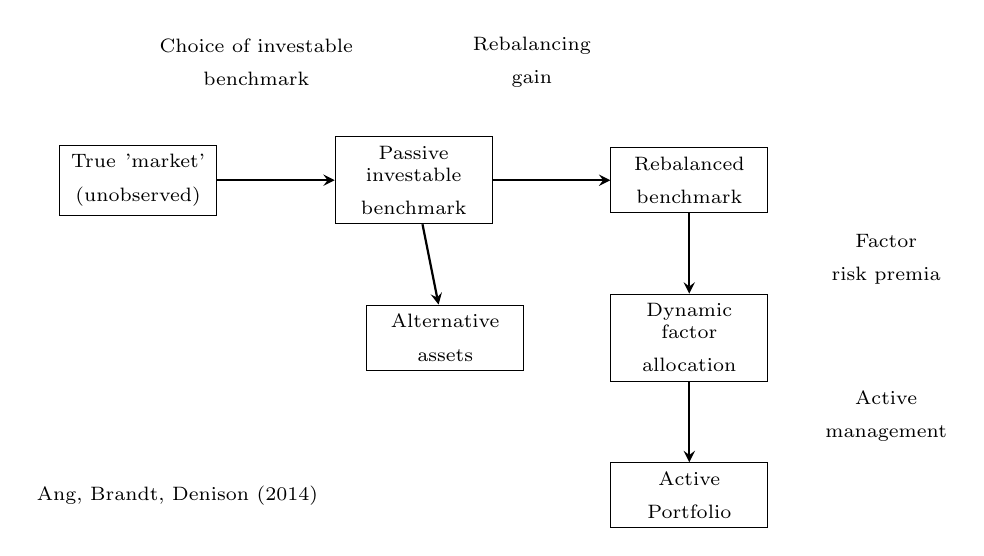
\begin{tikzpicture} 
%\draw[very thin, color = gray](0, 0) grid (12, 6);
\tikzstyle{block} = [draw, rectangle, text width = 5em, 
  text centered, minimum height = 6mm, node distance = 5em];
\tikzstyle{line} = [draw, -stealth, thick]
\node [block] at (1.5, 4) (one) {\scriptsize True 'market' \\ (unobserved)};
\node [block] at (5, 4) (two) {\scriptsize Passive investable \\ benchmark};
\node [block] at (5.4, 2) (twoandhalf) {\scriptsize Alternative \\ assets};
\node [block] at (8.5, 4) (three) {\scriptsize Rebalanced \\ benchmark};
\node [block] at (8.5, 2) (four) {\scriptsize Dynamic factor \\ allocation};
\node [block] at (8.5, 0) (five) {\scriptsize Active \\ Portfolio};
\path [line] (one) -- (two);
\path [line] (two) -- (three);
\path [line] (two) -- (twoandhalf);
\path [line] (three) -- (four);
\path [line] (four) -- (five);
\node at (3, 5.5) [align = center]{\scriptsize Choice of investable \\ \scriptsize benchmark};
\node at (6.5, 5.5) [align = center]{\scriptsize Rebalancing \\ \scriptsize gain};
\node at (11, 3) [align = center] {\scriptsize Factor \\ \scriptsize risk premia};
\node at (11, 1) [align = center] {\scriptsize Active \\ \scriptsize management};
\node at (2, 0) [align = center] {\scriptsize Ang, Brandt, Denison (2014)};
\end{tikzpicture}
\end{frame} 

\begin{frame}{References and further reading}
\begin{itemize}
\item Ang, A, W.N. Goetmann and S.M. Schaefer (2009), "Evaluation of Active Management of the Norwegian Government Pension Fund",

\item Arnott, R,. J.C. Hsu and Philip Moore (2005, "Fundamental Indexation", Financial Analysts Journal", Vol 61 No. 2. pp 83-89

\item Bender J., R. Briand, D. Melas, R. Subramanian, (2013), 'Foundations for Factor Investing", MSCI Research Insight. 

\item Dalio, R., B. Prince, G. Jensen, "Our Thoughts about Risk Parity and All Weather, Bridgewater Daily Observations" September 16 2015.

\item De Bondt, W. R. Thaler, (1995), "Does the Stock Market Overreact?", Journal of Finance, vol 40, No 3, 793-803 

\end{itemize}
\end{frame}

\begin{frame}{References cont.}
\begin{itemize}
\item Fama E.F, K.R. French, (1992), "The Cross Section of Expected Stock Returns", Journal of Finance, 47, 427-465

\item Fama E.F, K.R. French, (1993), "Common Risk Factors in the Returns on Stock and Bonds", Journal of Finance, 53, 1131-1147

\item Jagadesh N., S. Titman, (1993), "Returns to Buying Winners and Selling Losers: Implications for Stock Market Efficiency", Journal of Finance, Vol 48, No, 1, 65 -  91

\item Malkiel B., (1995), "Returns from Investing in Equity Mutual Funds 1971 to 1991", Journal of Finance, 50, 549-572

\item Podkaminer, E. (2013), Risk Factors as Building Blocks for Portfolio Diversification: the Chemistry of Asset Allocation, CFA Institute. 

\item Ross, S. (1976), "The Arbitrage Theory of Capital Asset Pricing", Journal of Economic Theory, 13 (3), 341-360

\end{itemize}
\end{frame}

\begin{frame}{Reading}
\begin{center}
\includegraphics[height = 3.0in]{factorbook}
\end{center}
\end{frame}
\end{document}
